\documentclass[tikz,border=3mm]{standalone}
\begin{document}
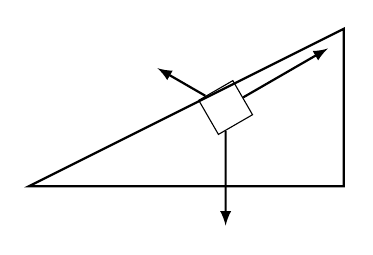
\begin{tikzpicture}
  % Define the inclined plane
  \draw[thick] (0,0) -- (4,2) -- (4,0) -- cycle;
  
  % Define the position and size of the cube
  \node[draw, rectangle, minimum size=0.5cm, rotate=30] (cube) at (2.5,1) {};
  
  % Define the forces
  \draw[-latex, thick] (cube) -- ++(0,-1.5) node[midway,right] {}; % gravity
  \draw[-latex, thick] (cube) -- ++(30:1.5) node[midway,right] {}; % normal force
  \draw[-latex, thick] (cube) -- ++(150:1) node[midway,right] {}; % frictional force
\end{tikzpicture}
\end{document}